\documentclass[9pt,pdf,hyperref={unicode}]{beamer}
\beamertemplatenavigationsymbolsempty
\usepackage{float}
\floatstyle{boxed} 
\restylefloat{figure}
\setbeamertemplate{blocks}[rounded=true, shadow=false]
\setbeamertemplate{footline}[page number]
\usepackage{multicol}
\usepackage{subfig}
\usefonttheme{serif}
\usepackage{amsfonts}
\usepackage[utf8]{inputenc}
\usepackage[english, russian]{babel}
\usepackage{amsmath,mathrsfs,mathtext}
\usepackage{graphicx, epsfig}
\usepackage{caption}
\usepackage{subfig}
\usepackage{amsmath, bm}
\usepackage{amssymb}
\usepackage{yfonts}
\usepackage{comment}

\usepackage{tabularx}

\usepackage{tikz}

\DeclareMathOperator*{\argmin}{arg\,min}
\DeclareMathOperator*{\argmax}{arg\,max}

\makeatletter
\let\@@magyar@captionfix\relax
\makeatother

\usetheme{Boadilla}
\usecolortheme{seahorse}


\setbeamertemplate{enumerate items}[circle]

\setbeamersize{text margin left=1.5em, text margin right=1.5em}

\usepackage{ragged2e}
% цветовая схема

\title[Ансамбль локальных моделей]
{Анализ свойств ансамбля локально
аппроксимирующих моделей}
\author[Исламов Р.\ И.]{\Large Исламов Рустем Ильфакович}
\institute[]{\large Московский физико-технический институт\\
~\\

Консультант: Грабовой А.\ В.\\
Эксперт:   Стрижов В.\ В.
}

\date{30 апреля 2020 г.}
%----------------------------------------------------------------------------------------------------------
\begin{document}
%----------------------------------------------------------------------------------------------------------
\begin{frame}
\titlepage
\end{frame}

%----------------------------------------------------------------------------------------------------------


\begin{frame}
\frametitle{Цель работы --- анализ свойств ансамбля локальных моделей} 


\begin{block}{Задача}
Аппроксимация данных, в которых данные порождены несколькими источниками
\end{block}


\begin{block}{Предлагаемое решение}
Построение универсальной модели в виде ансамбля локальных
моделей
\end{block}

\begin{block}{Требования к универсальному аппроксиматору}
\begin{itemize}
    \item Локальный модели должны быть простыми
    \item Локальные модели должны аппроксимировать разные подмножества объектов
    
\end{itemize}
\end{block}

\end{frame}

\begin{frame}{Список литературы}
	\begin{enumerate}
	\justifying
		\item \textit{V. V. Strijov A. V. Grabovoy.} Prior distribution choices for a mixture of experts. Machine learning and data analysis, 2020.
		

		\item \textit{Christopher M. Bishop.} Pattern Recognition and Machine Learning. SPRINGER NATURE, 2011.
 
		
		\item \textit{Павлов К.В.}  Выбор многоуровневых моделей в задачах классификации, 2012
		
		\item \textit{Esen Y.S., Wilson J., Gader P.D.}  Twenty Years of Mixture of Experts. IEEE Transactions on Neural Networks and Learning Systems. 2012. Issues. 23. No 8. P. 1177-1193.
		
	\end{enumerate}
\end{frame}



\begin{frame}{Постановка задачи построения ансмабля}
\begin{block}{Выборка}
Матрица признаков $\mathbf{X} \in \mathbb{R}^{N\times n}$ и выборка $\mathfrak{D} = \{(\mathbf{x}_i, \mathrm{y}_i): i \in \mathcal{I}\}$.
\end{block}
\begin{block}{Гипотеза порождения данных}
Выборка порождена $K$ источниками. Это предположение индуцирует разибение множества индексов $\mathcal{I}$ на $K$ непересекающихся подмножеств $\mathcal{I}_k$:
    \[\mathcal{I} = \bigsqcup_{k=1}^K \mathcal{I}_k.\]
Разбиение $\mathcal{I}$ индуцирует разбиение выборки данных $\mathfrak{D}$ и множества объектов~$\Omega$:
    \[\mathfrak{D} = \bigsqcup_{k=1}^K \mathfrak{D}_k, \qquad \Omega = \bigsqcup_{k=1}^K \Omega_k. \]
\end{block}
    
\end{frame}


\begin{frame}{Ансамбль локальных моделей}
    \begin{block}{Определение}
            Модель $ \mathrm{g}_k$ называется локальной, если она аппроксимирует подвыборку 
            \[\mathfrak{D}_k = \{(\mathbf{x}_i, \mathrm{y}_i): i \in \mathcal{I}_k\}.\]
    
    \end{block}

В данной работе каждая локальная модель является линейной. Локальные модели объединены в ансамбль локальных моделей. 
    \begin{block}{Определение}
        Ансамбль локальных моделей — мультимодель, определяющая правдоподобие веса $\pi_k$аждой локальной модели $\mathrm{g}_k$ на признаковом описании объекта $\mathbf{x}$.
\[\mathrm{f} = \sum\limits_{k=1}^K \pi_k \mathrm{g}_k(\mathbf{x}, \mathbf{w}_k), \qquad \pi_k(\mathbf{x}, \mathbf{V}): \mathbb{R}^{n\times |\mathbf{V}|}\rightarrow [0,1], \qquad \sum_{k=1}^K \pi_k(\mathbf{x}, \mathbf{V}) = 1, \]
где $\mathrm{f}$ --- ансамбль локальных моделей, $\mathrm{g}_k$ --- локальная модель,  $\pi_k$ --- шлюзовая функция, $\mathbf{V}$ --- параметры шлюзовой функции.

    \end{block}
\end{frame}

\begin{frame}{Расстояние между локальными моделями}
\begin{block}{Определение}
    Расстояние между локальными моделями равно выборочному коэффициенту корреляции Пирсона на выборке $\mathbf{X}$ и вычисляется по формуле
    
    \[\rho(\mathrm{g}_i, \mathrm{g}_j) = \frac{\sum\limits_{l=1}^N \left(\mathrm{X}_{il} - \overline{\mathrm{X}}_{i}\right)\left(\mathrm{X}_{jl} - \overline{\mathrm{X}}_{j}\right)}{\sqrt{\sum\limits_{l=1}^N \left(\mathrm{X}_{jl} - \overline{\mathrm{X}}_{j}\right)^2 \sum\limits_{l=1}^N \left(\mathrm{X}_{jl} - \overline{\mathrm{X}}_{j}\right)^2}}, \]
    $\mathrm{X}_{il} = (\mathbf{X}\mathbf{w}_i)_l, \mathrm{X}_{jl} = (\mathbf{X}\mathbf{w}_j)_l, \overline{\mathrm{X}}_i = \frac{1}{N}\sum\limits_{l=1}^N \mathrm{X}_{il}, \overline{\mathrm{X}}_i = \frac{1}{N}\sum\limits_{l=1}^N \mathrm{X}_{il}, \mathbf{w}_i, \mathbf{w}_j$~---~параметры локальных моделей~$\mathrm{g}_i$, $\mathrm{g}_j$.
    
\end{block}
\begin{block}{Цель введения расстояния}
Локальные модели должны быть независимыми, расстояние между ними должно быть близко к нулю.
\end{block}
    
\end{frame}

\begin{frame}{Базовый эксперимент}
\begin{block}{Цель базового эксперимента}
Показать, что выборка, порожденная несколькими источниками, плохо аппроксимируется одной моделью.
\end{block}\\
~\\
\begin{minipage}[t]{0.49\textwidth} 
   \begin{center}
   Данные первого эксперимента
   \[\mathbf{y} = \begin{pmatrix}
    \mathrm{y}_1\\
    \mathrm{y}_2
    \end{pmatrix}, \qquad\mathbf{X} = \begin{pmatrix}
    \mathrm{x}_1 & 0\\
    0 & \mathrm{x}_2
    \end{pmatrix}.\]
    \[\mathrm{y}_m = \alpha_{m}\mathrm{x}_m+ \varepsilon, \qquad \varepsilon \in \mathcal{N}(0, 1).\]
    \end{center}
    \end{minipage}%%%%%%%%%%%%%%%%%%%%%%%%%%%%
    \begin{minipage}[t]{0.49\textwidth} 
    \begin{center}
    Данные второго эксперимента
   \[\mathbf{y} = \begin{pmatrix}
    \mathrm{y}_1\\
    \mathrm{y}_2
    \end{pmatrix}, \qquad\mathbf{X} = \begin{pmatrix}
    \mathrm{x}_1 & \varepsilon_1\\
    \varepsilon_2 & \mathrm{x}_2
    \end{pmatrix}.\]
    \[\mathrm{y}_m = \alpha_{m}\mathrm{x}_m+ \varepsilon,\] 
    \[\varepsilon_{1,2} \in \mathcal{N}(0,1) \qquad \varepsilon \in \mathcal{N}(0, 1).\]
   \end{center}
    
    
    \end{minipage}  
\end{frame}



\begin{frame}{Результаты базового эксперимента}

  \begin{minipage}[t]{0.49\textwidth} 
    \begin{center}
    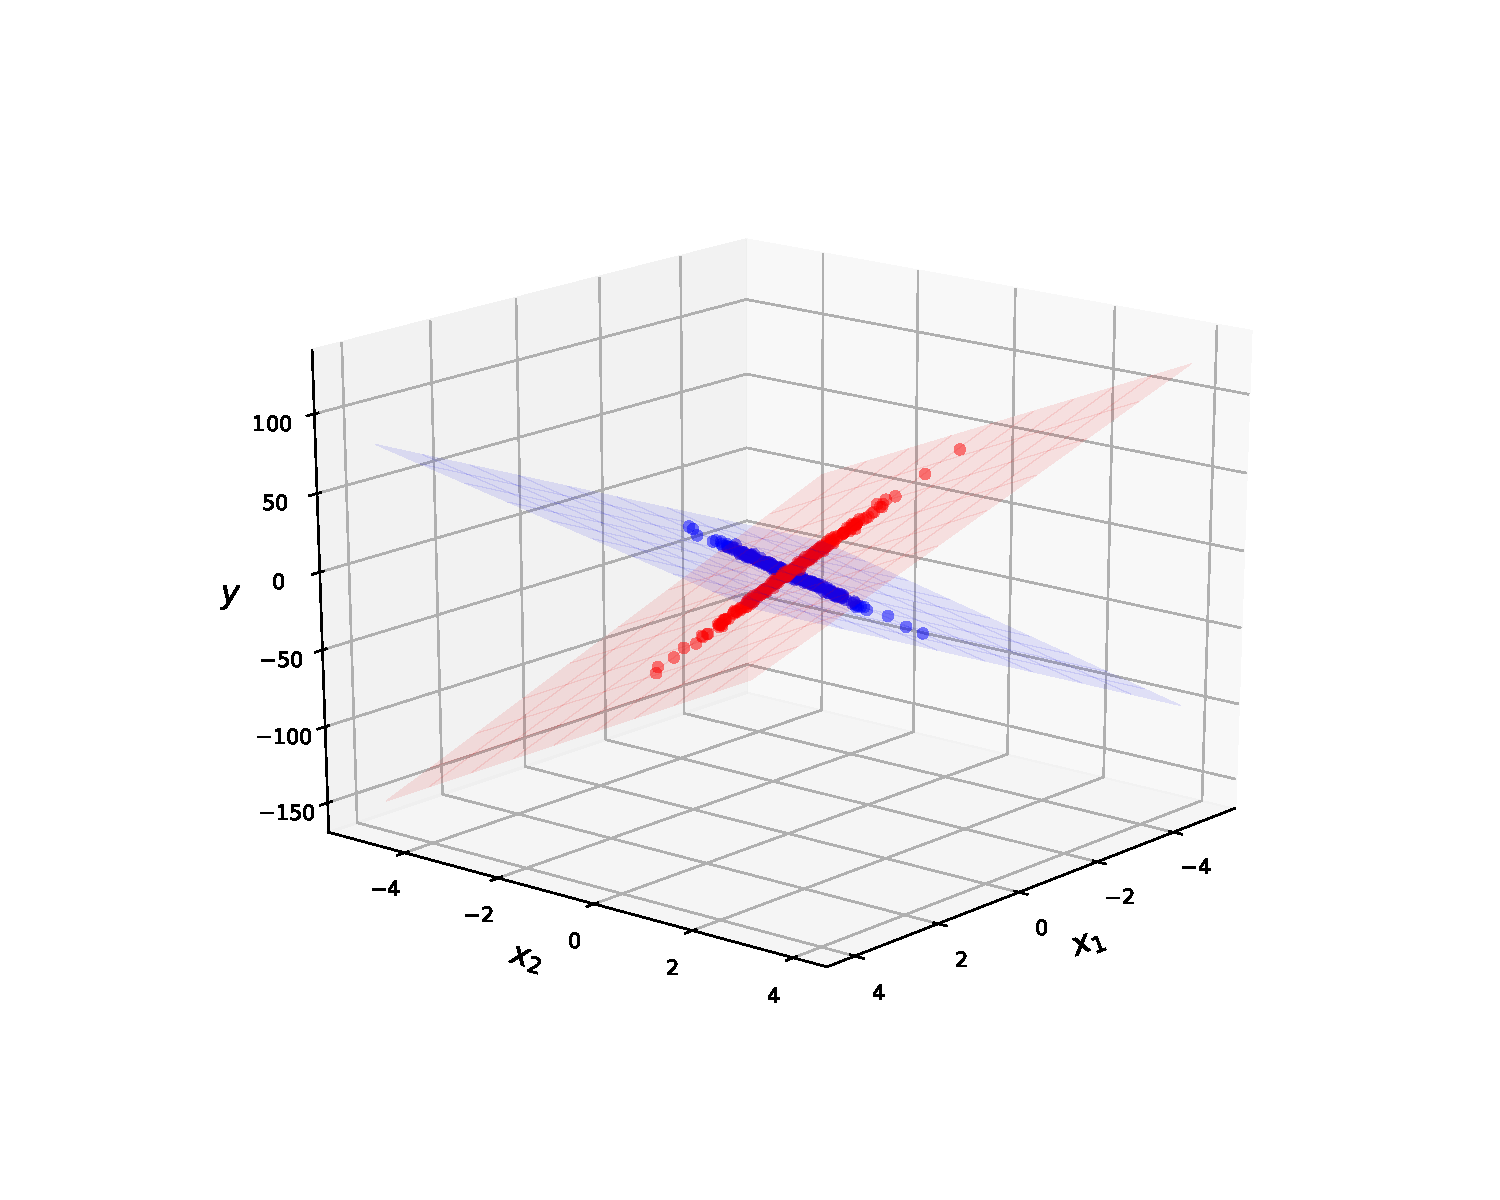
\includegraphics[width=0.95\linewidth]{experiment1-zeros.pdf}
    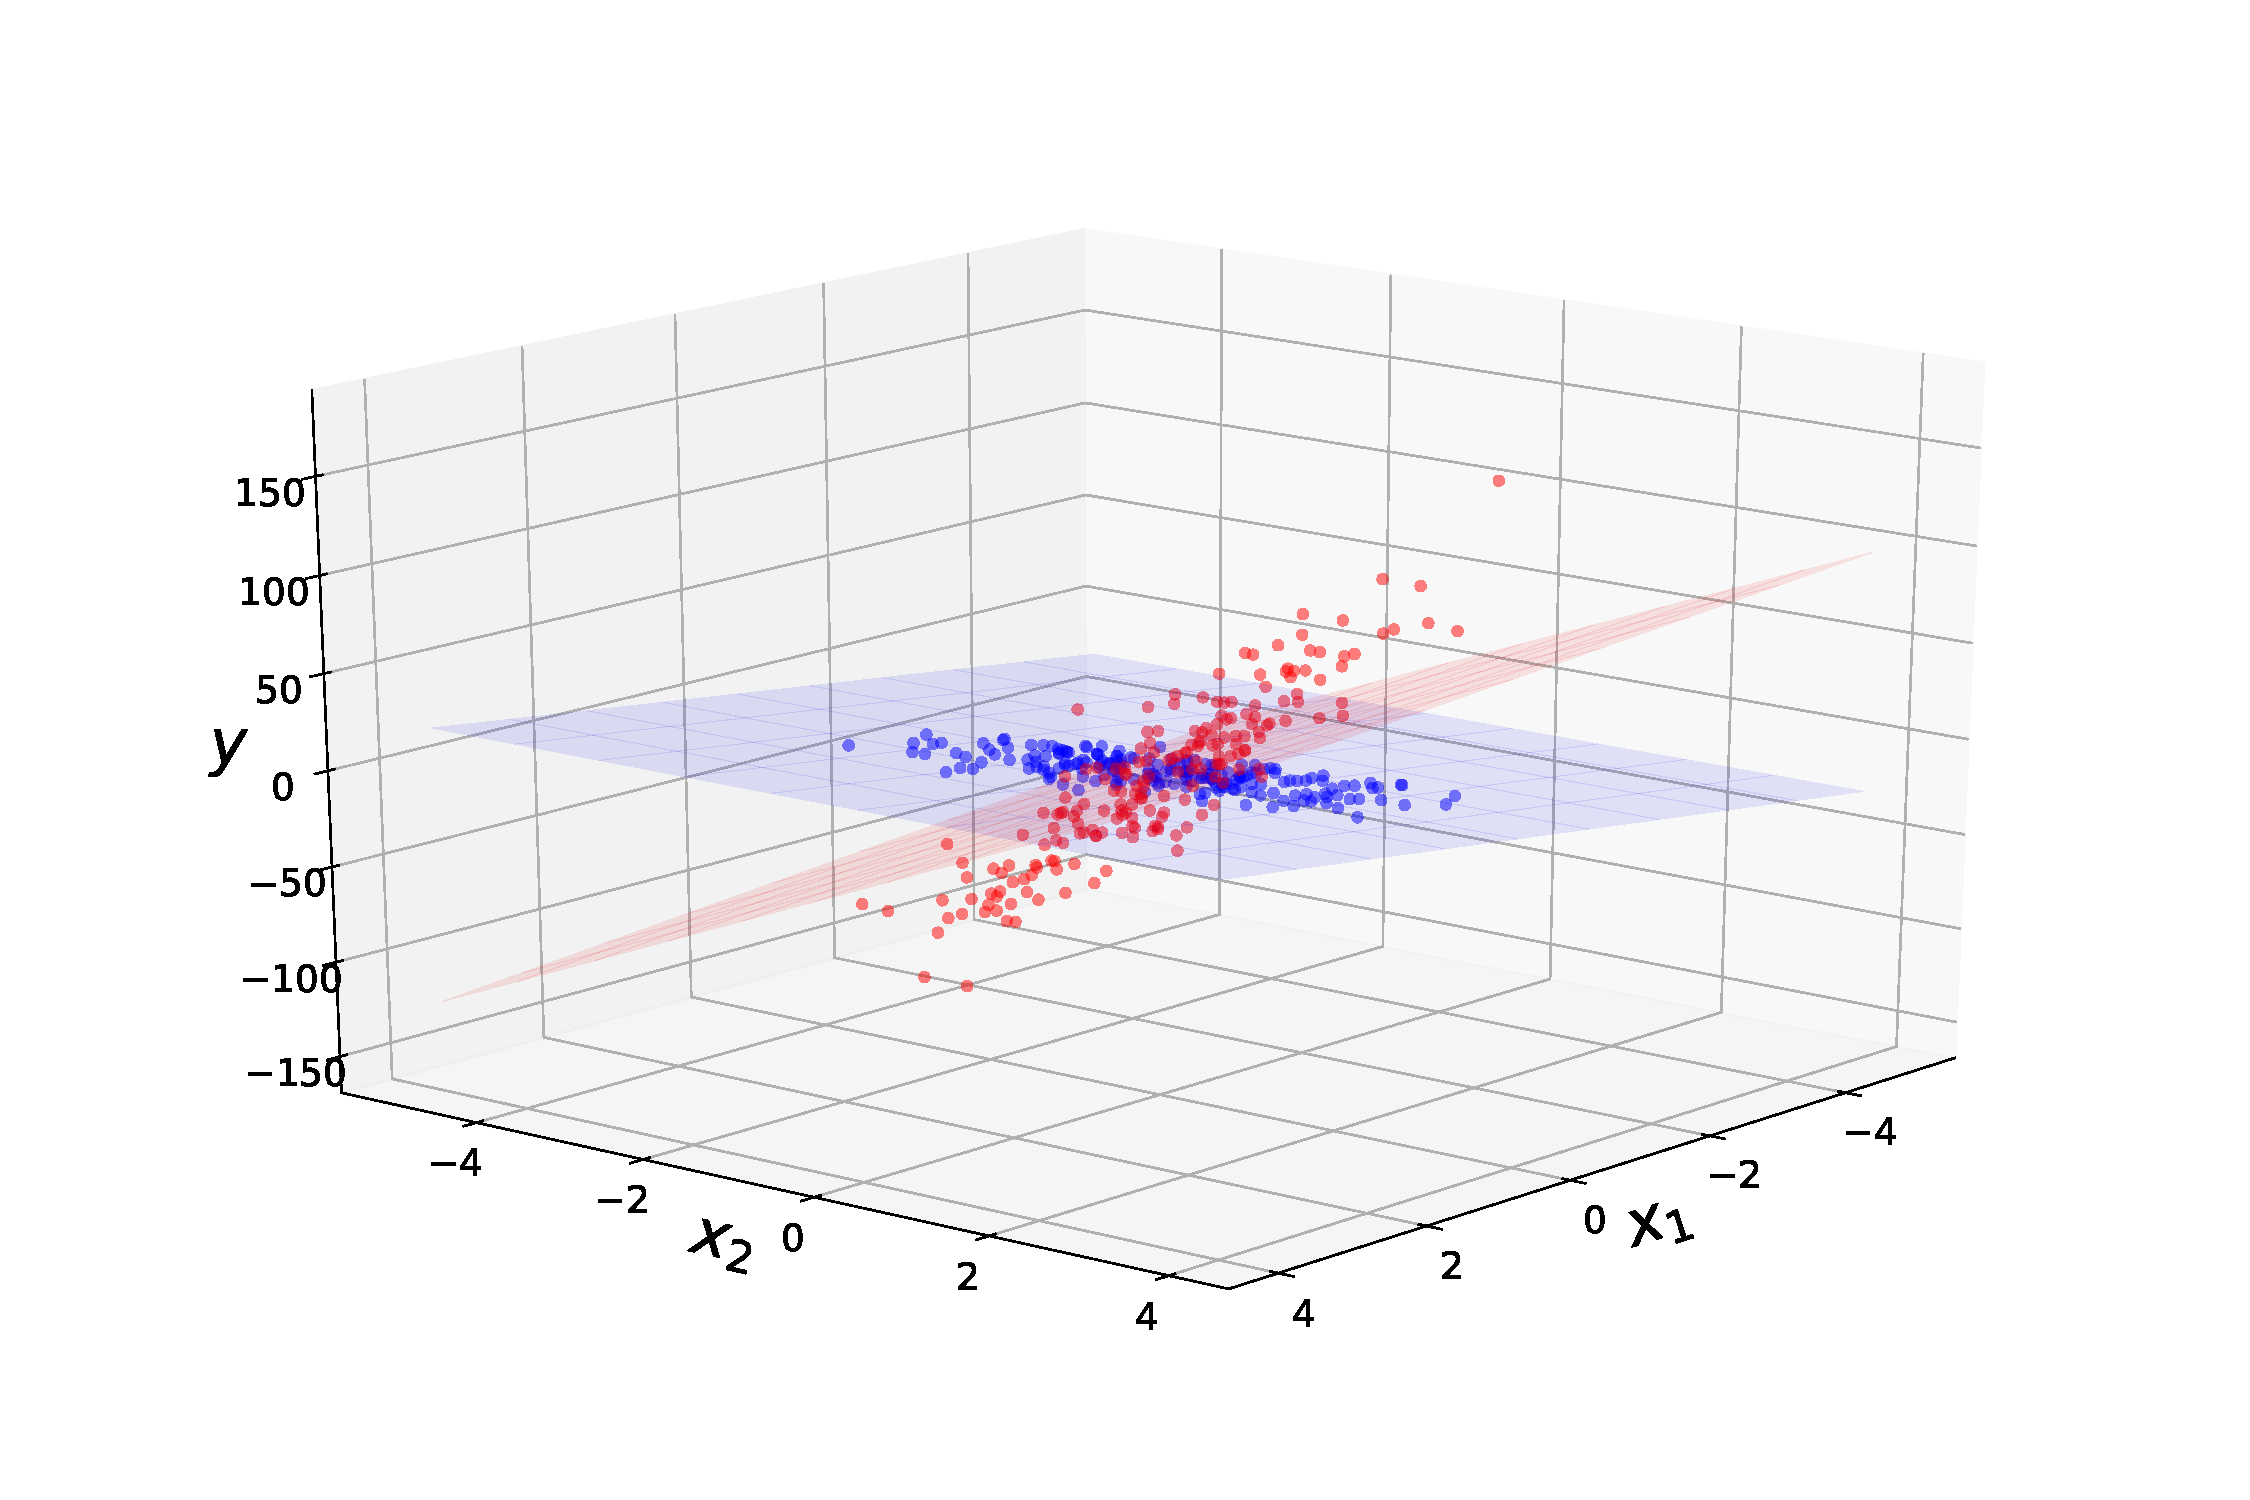
\includegraphics[width=0.95\linewidth]{experiment1-random.pdf}  \end{center}
    \end{minipage}%%%%%%%%%%%%%%%%%%%%%%%%%%%%
    \begin{minipage}[t]{0.49\textwidth} 
    \begin{center}
    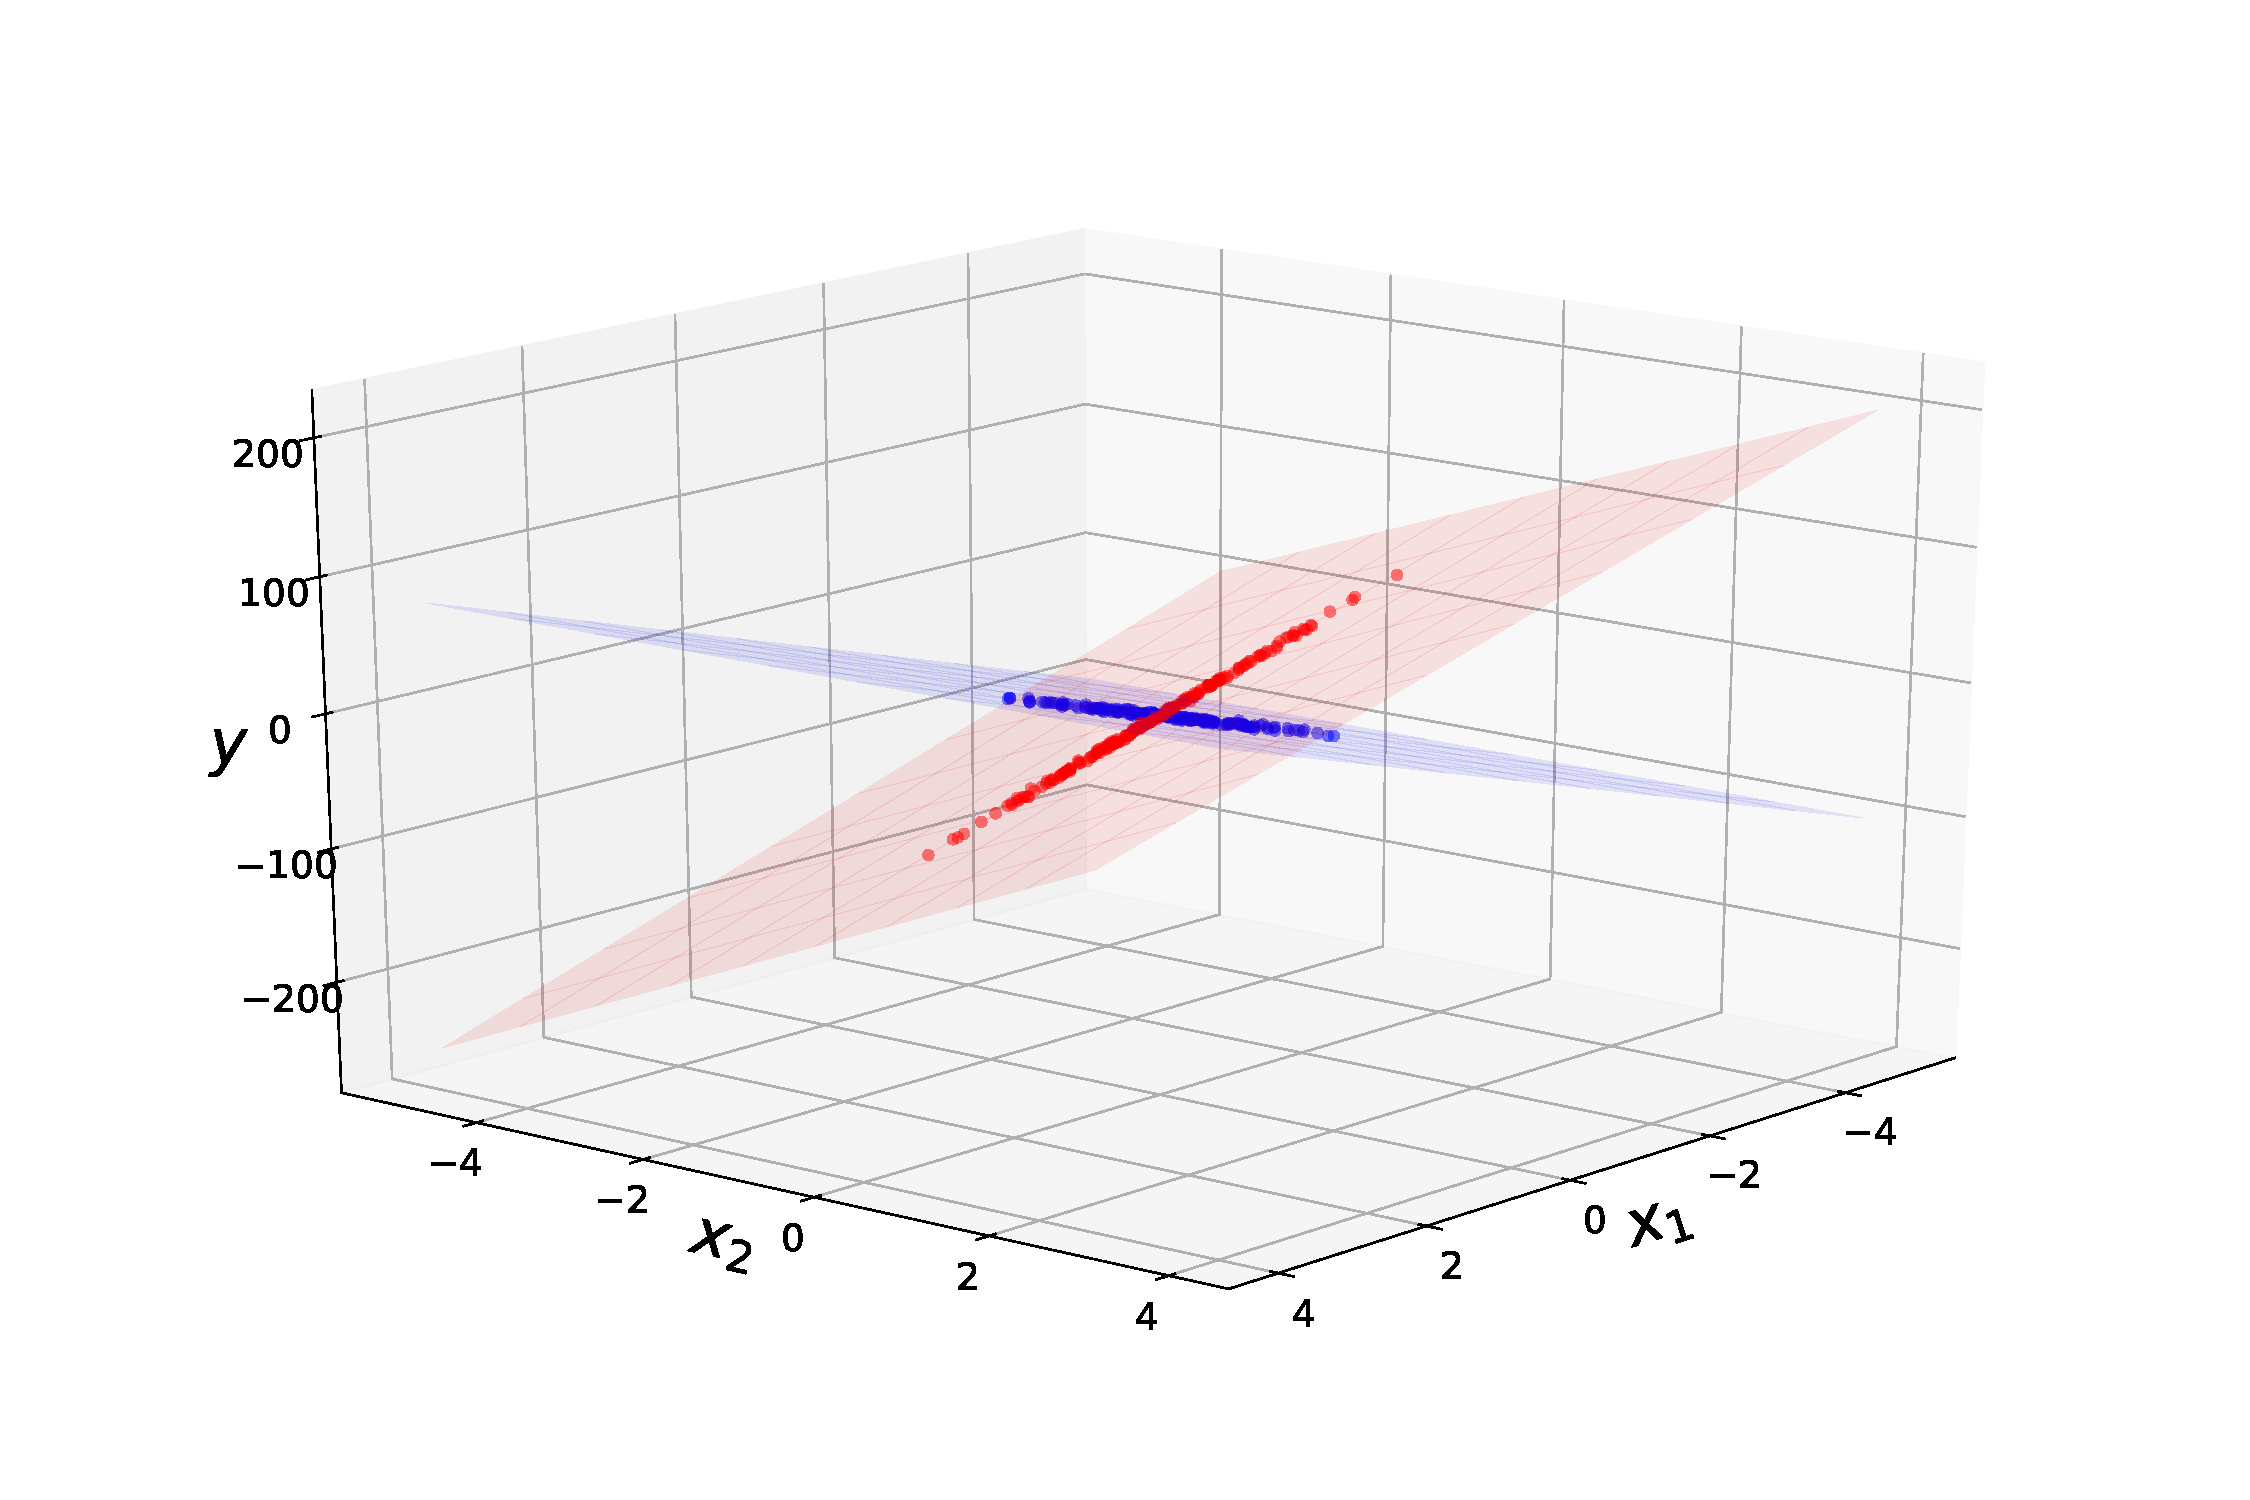
\includegraphics[width=0.95\linewidth]{experiment2-zeros.pdf}
    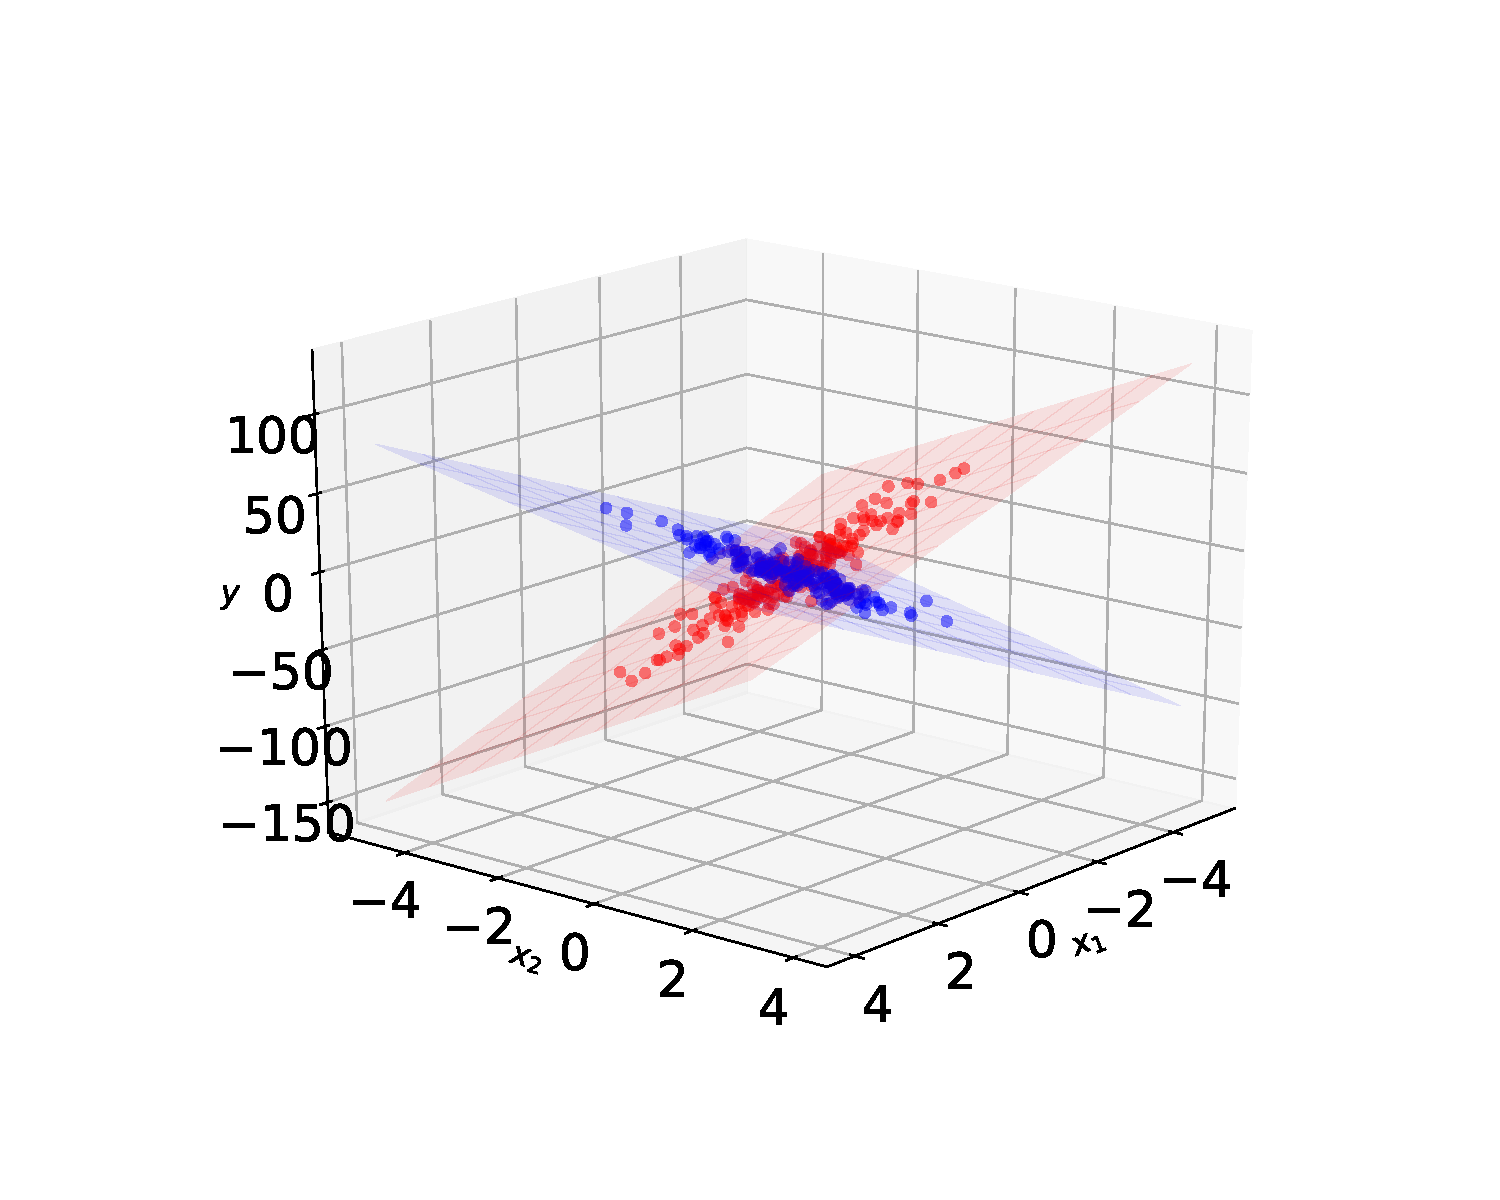
\includegraphics[width=0.95\linewidth]{experiment2-random.pdf}  \end{center}
    \end{minipage}
    Ансамбль локальных моделей лучше аппроксимирует выборку, порожденную несколькими источниками.
\end{frame}

\begin{frame}{Исследование расстояния между моделями на синтетической выборке}

Выборка для эксперимента
$\mathbf{y} = \begin{pmatrix}
\mathrm{y}_1\\
\mathrm{y}_2
\end{pmatrix},  \mathbf{\hat{X}} = \begin{pmatrix}
\mathrm{x}_1 & \varepsilon_1\\
\varepsilon_2 & \mathrm{x}_2
\end{pmatrix},$ где $\varepsilon_1, \varepsilon_2 \in \mathcal{N}(0,\sigma)$.

\begin{center}
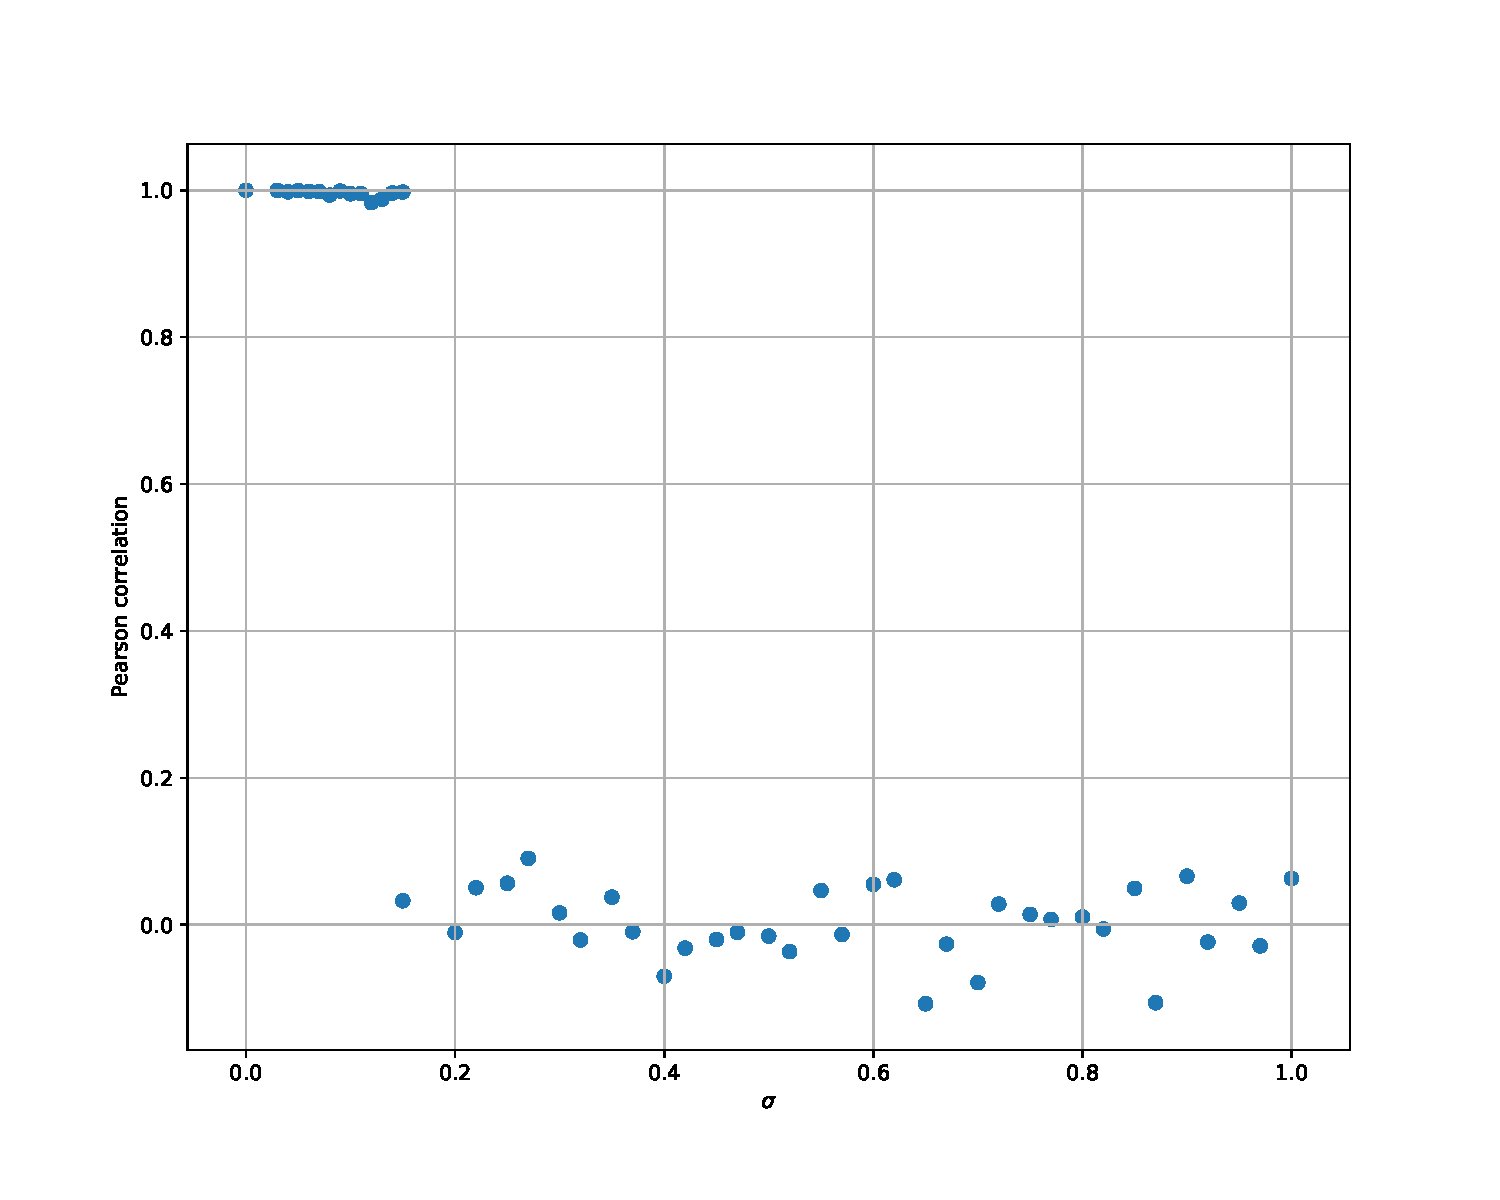
\includegraphics[width=0.6\linewidth]{Pearson_cor_sigma_synthetic.pdf}
\end{center}
При параметре шума $\sigma$ меньшем порогового значения локальные модели практически одинаковы, при $\sigma$ большем порога локальные модели независимы.

\end{frame}

\begin{frame}{Исследование расстояния между моделями на реальных выборках}
    
    Выборка для эксперимента
$\tilde{\mathbf{y}} = \begin{pmatrix}
\mathbf{y}_b\\
\mathbf{y}_s
\end{pmatrix} \in \mathbb{R}^{673}, \qquad \tilde{\mathbf{X}} = \begin{pmatrix}
\mathbf{X}_b\\
\mathbf{X}_s ~~\mathbf{\mathcal{E}}
\end{pmatrix} \in \mathbb{R}^{673\times 13}.$

\begin{center}
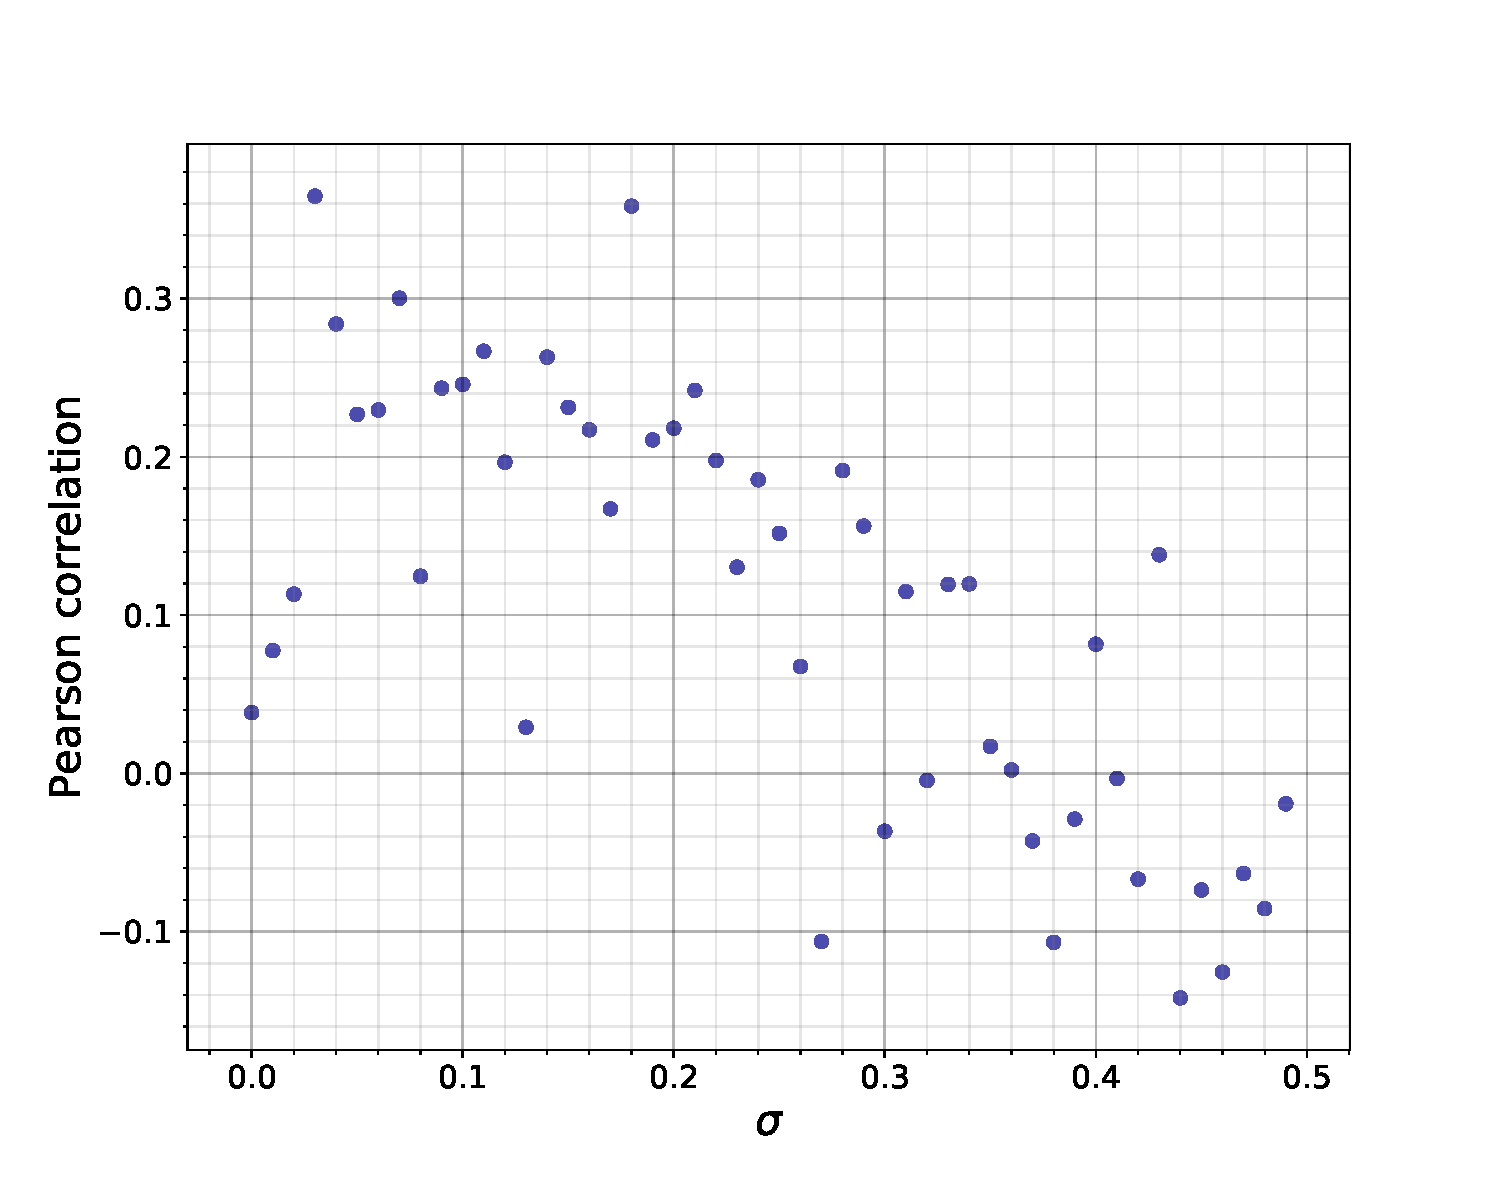
\includegraphics[width=0.6\linewidth]{Pearson_cor_sigma_boston_and_servo.pdf}
\end{center}
При увеличении параметра шума есть тенденция к уменьшению расстояния между локальными моделями, они становятся более независимыми. 
\end{frame}





\begin{frame}{Заключение}
    \begin{block}{Полученные результаты}
    \begin{itemize}
        \item Качество аппроксимации выборки, порожденной несколькими источниками, при использовании ансамбля локальных моделей выше, чем у одной модели
        \item При увеличении параметра шума модели становятся независимыми
    \end{itemize}
    \end{block}
    \begin{block}{Дальнейшие исследования}
    \begin{itemize}
        \item Исследование оптимального количества локальных моделей в ансамбле
        \item Использование расстояния между локальными моделями как регуляризатор 
    \end{itemize}
    \end{block}
\end{frame}





\end{document}
  